\documentclass[a4paper, fontsize=11pt]{scrartcl} % A4 paper and 11pt font 
\usepackage[a4paper,left=3cm,right=2cm,top=2.5cm,bottom=2.5cm]{geometry}

\usepackage[T1]{fontenc} % Use 8-bit encoding that has 256 glyphs
\usepackage{fourier} % Use the Adobe Utopia font for the document - comment this line to return to the LaTeX default
\usepackage[spanish]{babel} % Spanish language/hyphenation
\selectlanguage{spanish}
\usepackage[utf8]{inputenc}
\usepackage{amsmath,amsfonts,amsthm} % Math packages
\usepackage{graphicx} % The graphicx package
\usepackage{placeins}
\usepackage{caption}
\usepackage{subcaption}


\usepackage{listings} % Insert Scripts
\usepackage{color} %red, green, blue, yellow, cyan, magenta, black, white
\definecolor{mygreen}{RGB}{28,172,0} % color values Red, Green, Blue
\definecolor{mylilas}{RGB}{170,55,241}

\lstset{language=Matlab,%
	%basicstyle=\color{red},
	breaklines=true,%
	morekeywords={matlab2tikz},
	keywordstyle=\color{blue},%
	morekeywords=[2]{1}, keywordstyle=[2]{\color{black}},
	identifierstyle=\color{black},%
	stringstyle=\color{mylilas},
	commentstyle=\color{mygreen},%
	showstringspaces=false,%without this there will be a symbol in the places where there is a space
	numbers=left,%
	numberstyle={\tiny \color{black}},% size of the numbers
	numbersep=9pt, % this defines how far the numbers are from the text
	emph=[1]{for,end,break},emphstyle=[1]\color{red}, %some words to emphasise
	%emph=[2]{word1,word2}, emphstyle=[2]{style},    
}

\usepackage{sectsty} % Allows customizing section commands
%\allsectionsfont{\centering \normalfont\scshape} % Make all sections centered, the default font and small caps

\usepackage{fancyhdr} % Custom headers and footers
\pagestyle{fancyplain} % Makes all pages in the document conform to the custom headers and footers
\fancyhead{} % No page header - if you want one, create it in the same way as the footers below
\fancyfoot[L]{} % Empty left footer
\fancyfoot[C]{} % Empty center footer
\fancyfoot[R]{\thepage} % Page numbering for right footer
\renewcommand{\headrulewidth}{0pt} % Remove header underlines
\renewcommand{\footrulewidth}{0pt} % Remove footer underlines
\setlength{\headheight}{13.6pt} % Customize the height of the header

\numberwithin{equation}{section} % Number equations within sections (i.e. 1.1, 1.2, 2.1, 2.2 instead of 1, 2, 3, 4)
\numberwithin{figure}{section} % Number figures within sections (i.e. 1.1, 1.2, 2.1, 2.2 instead of 1, 2, 3, 4)
\numberwithin{table}{section} % Number tables within sections (i.e. 1.1, 1.2, 2.1, 2.2 instead of 1, 2, 3, 4)

%\setlength\parindent{0pt} % Removes all indentation from paragraphs - comment this line for an assignment with lots of text

\newenvironment{myalign}{\par\nobreak\large\noindent\align}{\endalign} %Altering fontsize in equations globally

%----------------------------------------------------------------------------------------
%	TITLE SECTION
%----------------------------------------------------------------------------------------

\newcommand{\horrule}[1]{\rule{\linewidth}{#1}} % Create horizontal rule command with 1 argument of height

\title{	
	\normalfont \normalsize 
	\textsc{Master en Automática y Robótica - UPM} \\ [25pt] % Your university, school and/or department name(s)
	\horrule{0.5pt} \\[0.4cm] % Thin top horizontal rule
	\huge Introducción a los Procesos Estocásticos \\ % The assignment title
	\horrule{2pt} \\[0.5cm] % Thick bottom horizontal rule
}

\author{Jorge Camarero Vera - 07052} % Your name

\date{\normalsize\today} % Today's date or a custom date

\begin{document}
	\maketitle
	
	\section{Caracterización de Procesos Estocásticos}
	
	Caracterizar un proceso estocástico de los datos en \textit{datos\_tema\_2.mat}. Primero habrá que calcular medias, varianzas, filtrar si es necesario y verificar si la varianza es pequeña. Si es así el proceso es estacionario. Finalmente al calcular las covarianzas si estas son muy pequeñas el proceso será ergódico. Por último, si el proceso es ergódico, ver si la media, varianza y covarianza de cualquier realización coincide. Una vez decidido que es ergódico, ver si la media, varianza y covarianza de cualquier realización coincide También habrá que averiguar si los datos son ruido blanco.
	
	\subsection{Presentación de los datos}
	
	Un proceso estocástico es una familia indexada de variables aleatorias reales $\left\lbrace x(t); t\in I \right\rbrace$, definidas sobre un mismo espacio muestral con una misma función de probabilidad $\left( \Omega, P(\Omega),p \right) $. En donde:
	
	\begin{itemize}
		\item I(Conjunto índice) puede ser
			\begin{itemize}
				\item Discreto $\Longrightarrow$ Proceso discreto.
				\item Continuo $\Longrightarrow$ Proceso continuo.
				\item Control estocástico: tiempo.
			\end{itemize}
		\item $\Omega$: Espacio Muestral
		\item $P(\Omega)$: Conjunto de las Partes de $\Omega$ (sucesos).
		\item $p$: Probabilidad.
	\end{itemize}
	
	En este ejercicio los datos pertenecen al ámbito de los procesos estocásticos discretos, por lo que:
	
	\begin{itemize}
		\item Notación simplificada: $x(k)$
		\item Notación real: $x(k,r)$
		\item Para $k$ fijo $\Longrightarrow$ $x_k(r)$ variable aleatoria real.
		\item Para $r$ fijo $\Longrightarrow$ $x_r(k)$ secuencia de valores reales (trayectoria o realización del proceso).
	\end{itemize}
	
	Los datos que contiene el archivo \textit{datos\_tema\_2.mat} es una matriz de 2000x2000. Como no ha habido mayores indicaciones asumiré que las filas corresponden a valores de $k$ y las columnas a valores de $r$.
	
	Un ejemplo de representación tanto de la realización del proceso, Figura \ref{PlotXr}, como de la variable aleatoria real, Figura \ref{PlotXk}.
	
	\begin{figure}[h!]
		\centering
		\begin{subfigure}{0.5\textwidth}
			\centering
			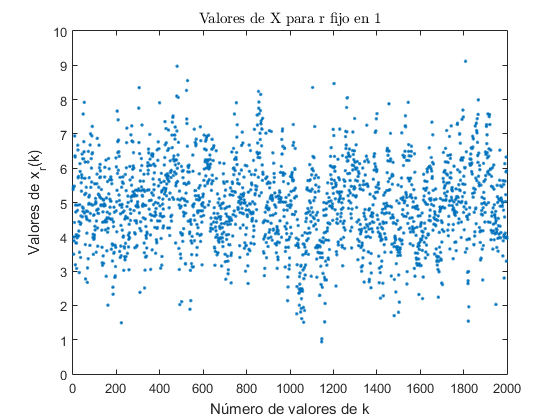
\includegraphics[width=1.0\linewidth]{images/PlotXr.PNG}
			\caption{Representación de $X_r(k)$}
			\label{PlotXr}
		\end{subfigure}%
		\begin{subfigure}{0.5\textwidth}
			\centering
			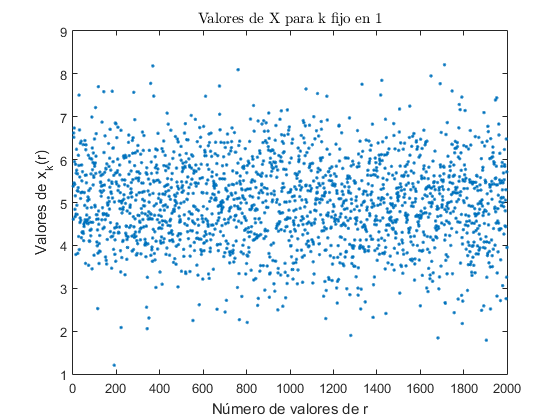
\includegraphics[width=1.0\linewidth]{images/PlotXk.PNG}
			\caption{Representación de $X_k(r)$}
			\label{PlotXk}
		\end{subfigure}
		\caption{Representación de los valores de $X_r(k)$ e $X_k(r)$}
		\label{Plots}
	\end{figure}
	\FloatBarrier
	
	\subsection{Caracterización de Procesos Estocásticos}
	
	Para la caracterización completa del proceso, se necesita conocer la función de densidad conjunta de las $N$ variables aleatorias. Como la caracterización de un proceso estocástico es muy costosa, por tanto, se recurre a caracterizaciones parciales más sencillas. La caracterización de primer orden considera sólo las distribuciones marginales, pero es insuficiente para los fines de control estocástico. La de segundo orden considera el primer orden y todos los pares de variables aleatorias.\\
	
	Se realizarán caracterizaciones parciales de segundo orden en base a momentos:\\
	
	\begin{description}
		\item[Media:] 
		\begin{myalign}
			\overline{x(k)}=E\left[x(k)\right] = \lim\limits_{n\rightarrow \infty}\dfrac{1}{n}\sum_{r=1}^{n}x(k,r)
		\end{myalign}
		\item[Varianza:]
		\begin{myalign}
			\sigma_x^2(k)=E\left[ \left( x(k)- \overline{x(k)}\right)^2 \right]
		\end{myalign}
		\item[Covarianza:]
		\begin{myalign}
			C_x(k_1,k_2)=E\left[ \left( x(k_1)-\overline{x(k_1)}\right) \left( x(k_2)-\overline{x(k_2)}\right) \right]
		\end{myalign}
		\item[Esperanza conjunta:]
		\begin{myalign}
			E_x(k_1,k_2)=E\left[ x(k_1)x(k_2) \right]
		\end{myalign}
		\item[Correlación:]
		\begin{myalign}
			\rho_x(k_1,k_2)=\dfrac{C_x(k_1,k_2)}{\sigma_x(k_1)\sigma_x(k_2)}
		\end{myalign}
	\end{description}
	
	Vamos a calcular las medias y varianzas de cada momento y representarlas en Figura \ref{Caracteristicas} , para ello se usará los métodos creados en la anterior entrega.\\
	
	\begin{lstlisting}
		for i = 1: 2000
		means(i) = Probability_Homework.mean(X(i,:));
		variances(i) = Probability_Homework.varianceUnBias(X(i,:));
		end
	\end{lstlisting}
	
	\begin{figure}[h!]
		\centering
		\begin{subfigure}{0.5\textwidth}
			\centering
			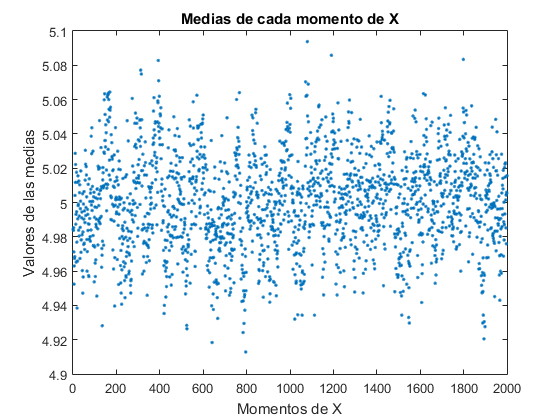
\includegraphics[width=1.0\linewidth]{images/Means.PNG}
			\caption{Representación de las medias}
			\label{Medias}
		\end{subfigure}%
		\begin{subfigure}{0.5\textwidth}
			\centering
			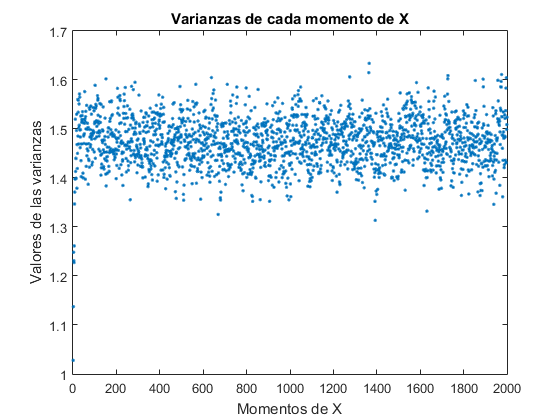
\includegraphics[width=1.0\linewidth]{images/Variances.PNG}
			\caption{Representación de las varianzas}
			\label{Varianzas}
		\end{subfigure}
		\caption{Representación de las características de X}
		\label{Caracteristicas}
	\end{figure}
	\FloatBarrier
	
	Al mirar las varianzas, se visualiza que al principio las varianzas van cambiando para después estabilizarse, por lo que se podrían filtrar esos primeros momentos. Ahora calculamos las covarianzas, esperanzas conjuntas y correlaciones de los datos, realizándolo entre el momento inicial, sí mismo y los siguientes.
	
	\begin{lstlisting}
	for i = 1:2000
	covariance = Probability_Homework.covarianceUnBias(X(1,:),X(i,:));
	covs(i) = covariance(1,2);
	R(i) = Probability_Homework.mean(X(1,:).*X(i,:));
	correlation = Probability_Homework.correlation(X(1,:),X(i,:));
	corrs(i) = correlation(1,2);
	end
	\end{lstlisting}
	
	\begin{figure}[h!]
		\centering
		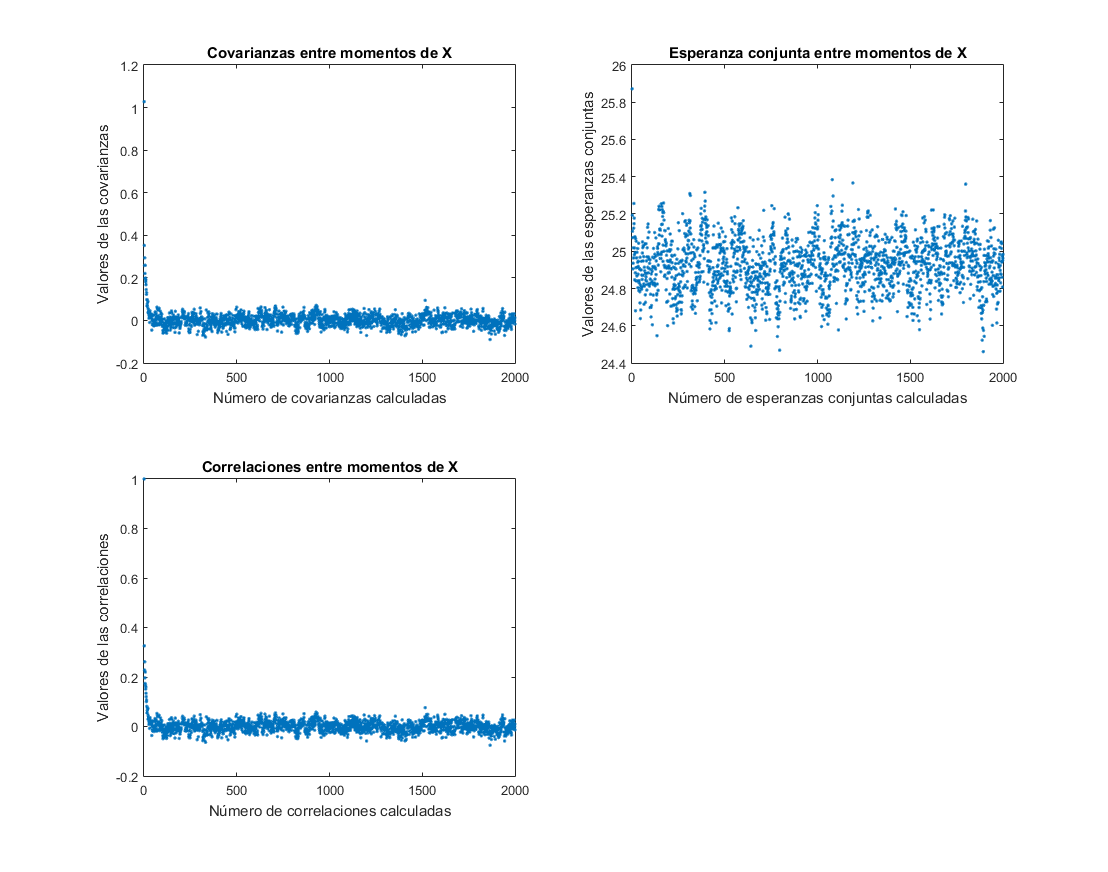
\includegraphics[width=1.0\linewidth]{images/caract.PNG}
		\caption{Representación de las características de X}
		\label{Caracteristicas2}
	\end{figure}
	\FloatBarrier
	
	Al igual que en las varianzas habría que filtrar los primeros valores. Y por tanto ya quedan definidas las características del proceso estocástico.\\
	
	Un proceso estocástico de segundo orden es aquel que tiene sus momentos de primer y segundo orden acotados, es decir:
	
	\begin{myalign}
		E\left[ x^2(k) \right] < \infty
	\end{myalign}
	
	\begin{lstlisting}
		for i = 1:2000
		R(i) = Probability_Homework.mean(X(i,:).*X(i,:));
		end
	\end{lstlisting}
	
	\begin{figure}[h!]
		\centering
		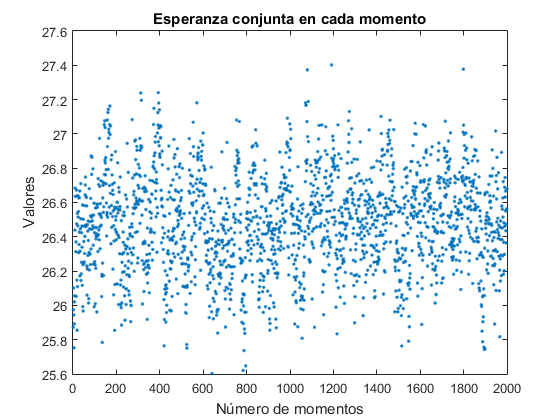
\includegraphics[width=1.0\linewidth]{images/Esperanzas.PNG}
		\caption{Esperanza conjunta en cada momento}
		\label{Esperanzas}
	\end{figure}
	\FloatBarrier
	
	Todos los valores están acotados, por lo que \textbf{el proceso estocástico es de segundo orden.}\\
	
	\subsubsection{Proceso Estocástico Estacionario}
	
	Ahora veremos si es un proceso estocástico estacionario. Un proceso estocástico $x(k)$ es \textit{estacionario en sentido estricto} cuando la función de densidad conjunta de cualquier subconjunto de las variables aleatorias del proceso es invariante ante un desplazamiento en k. Un proceso estocástico $x(k)$ es \textit{estacionario en sentido amplio} (o débil) cuando sus momentos de primer u segundo orden son invariantes ante un desplazamiento en $k$.\\
	
	Mirando las gráficas anteriores, Figuras \ref{Caracteristicas} y \ref{Caracteristicas2}, observamos que los valores son más o menos invariantes ante un desplazamiento de $k$, dentro de un pequeño margen de valores, por lo que \textbf{el proceso estocástico es estacionario.}
	
	\subsubsection{Proceso Ergódico}
	
	Un proceso estacionario de 2º orden es ergódico si  se verifica:
	
	\begin{myalign}
		\lim\limits_{N\rightarrow\infty}\sigma_s^2=0
		\label{ergodico}
	\end{myalign}
	
	Viendo en la Figura \ref{Caracteristicas2} las covarianzas entre momentos de X se llega a la conclusión de que \textbf{el proceso es ergódico}, ya que se cumple la ecuación (\ref{ergodico}), al tender las covarianzas a 0.
	
	\subsubsection{Caracterización Frecuencial}
	
	El espectro de potencia $S(\omega)$ de un proceso de 2º orden estacionario es la transformada de Fourier de su covarianza.
	
	\begin{myalign}
		S_x(\omega) = \sum_{i=-\infty}^{\infty}C_x(i)e^{-ji\omega T} \Leftrightarrow C_x(i)=\dfrac{T}{2\pi}\int_{-\pi/T}^{\pi/T}S_x(\omega)e^{ji\omega T}d\omega
	\end{myalign}
	
	Y teniendo en cuenta que la covarianza es par:
	
	\begin{myalign}
		\begin{split}
		S_x(\omega)	&=\sum_{i=-\infty}^{\infty}C_x(i)e^{-ji\omega T}=C_x(0)+\sum_{i=1}^{\infty}C_x(i)\left(e^{+ji\omega T}+e^{-ji\omega T}\right) =\\
					&= C_x(0)+2\sum_{i=1}^{\infty}C_x(i)cos(i\omega T)
		\end{split}
	\end{myalign}
	
	Para calcular la transformada de Fourier de las covarianzas empleo la función de MATLAB fft() quedando la Figura \ref{Caracterización Frecuencial}.
	
	\begin{lstlisting}
		for i = 1:2000
		covariance = cov(X(1,:),X(i,:));
		covs(i) = covariance(1,2);
		end
		Y = fft(covs);
		plot(linspace(1,2000,2000),abs(Y),'-');
	\end{lstlisting} 
	
	\begin{figure}[h!]
		\centering
		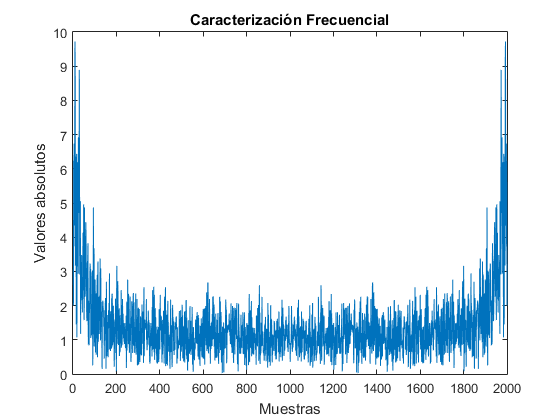
\includegraphics[width=1.0\linewidth]{images/FFT.PNG}
		\caption{Caracterización Frecuencial}
		\label{Caracterización Frecuencial}
	\end{figure}
	\FloatBarrier
	
	Vemos que la transformada de Fourier produce valores simétricos, por lo que nos podemos quedar con los valores de 1 a 1000, además como hemos dicho en anteriores apartados los primeros valores los podemos filtrar. Y quedaría Figura \ref{Caracterización Frecuencial Filtrada}.
	
	\begin{figure}[h!]
		\centering
		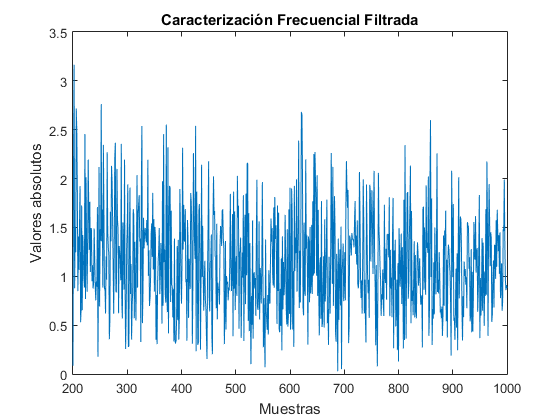
\includegraphics[width=1.0\linewidth]{images/FFTFiltrada.PNG}
		\caption{Caracterización Frecuencial Filtrada}
		\label{Caracterización Frecuencial Filtrada}
	\end{figure}
	\FloatBarrier
	
    Se muestra un valor más o menos constante en torno a 1. Además la definición de ruido blando es un proceso estacionario cuyo espectro de potencia es constante.
    
    \begin{myalign}
    	S_x(\omega)=cte
    \end{myalign}
    
    Por tanto \textbf{es un ruido blanco}. Para comparar vemos la caracterización frecuencial de un ruido blanco, Figura \ref{Espectro de Potencia del Ruido Blanco}.
	
	\begin{lstlisting}
		% Generacion de matriz 2000x2000 de ruido blanco
		y1 = wgn(2000,2000,0);
		for i = 1:2000
		covariance = cov(y1(1,:),y1(i,:));
		WNcovs(i) = covariance(1,2);
		end
		WN = fft(WNcovs);
		plot(linspace(1,2000,2000),abs(WN),'-');		
	\end{lstlisting}	
	
	\begin{figure}[h!]
		\centering
		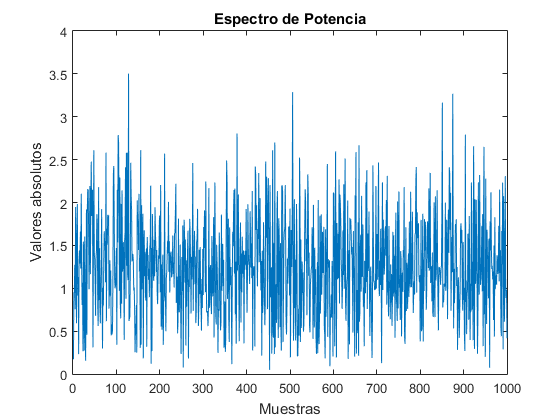
\includegraphics[width=1.0\linewidth]{images/WhiteNoise.PNG}
		\caption{Espectro de Potencia del Ruido Blanco}
		\label{Espectro de Potencia del Ruido Blanco}
	\end{figure}
	\FloatBarrier
	
	Vemos que tanto la Figura \ref{Caracterización Frecuencial Filtrada} como la Figura \ref{Caracterización Frecuencial Filtrada} se parecen bastante. Por lo que se puede decir que \textbf{el proceso es un ruido blanco}.
	
	\subsubsection{Calcular media, varianza y covarianza de cualquier realización}
	
	Para calcular la media, varianza y covarianza de cualquier realización ejecutamos  el algoritmo de abajo y obtenemos la Figura \ref{Características de las realizaciones}.
	
	\begin{lstlisting}
		for i = 1:2000
		means(i) = mean(X(:,i));
		variances(i) = var(X(:,i));
		covariance = cov(X(:,1),X(:,i));
		covsR(i) = covariance(1,2);
		end
	\end{lstlisting}
	
	\begin{figure}[h!]
		\centering
		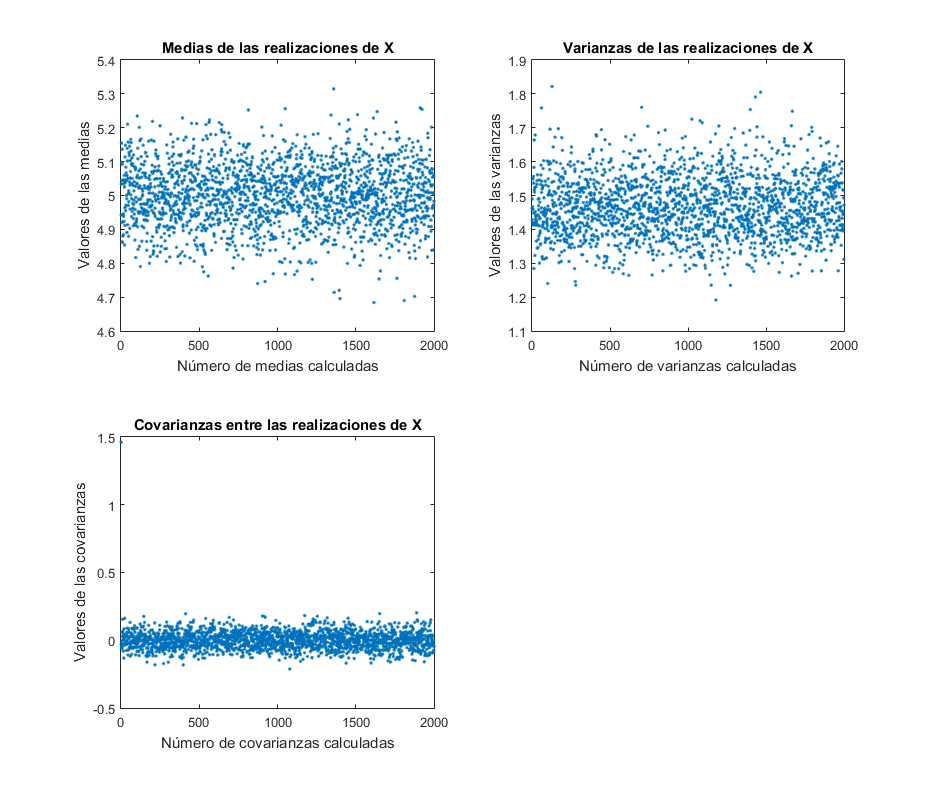
\includegraphics[width=1.0\linewidth]{images/Caract2.PNG}
		\caption{Características de las realizaciones}
		\label{Características de las realizaciones}
	\end{figure}
	\FloatBarrier
	
	Vemos que tienen \textbf{valores semejantes} (coincidentes) a los calculados en anteriores apartados. Lo que también concuerda con que el proceso estocástico sea ruido blanco.
	
\end{document}